\documentclass[a4paper]{article}

\usepackage[utf8]{inputenc}
\usepackage[english]{babel}
\usepackage{hyperref}
\usepackage{graphicx}
\usepackage{amsmath,amssymb,amsthm}
\usepackage{siunitx}
\usepackage{xcolor}
\usepackage{multicol}
\usepackage{caption}
\usepackage{appendix}
\usepackage{pdfpages}
\usepackage{fixltx2e}
\usepackage[version=4]{mhchem}
\usepackage{url}
\usepackage{subcaption}
\usepackage{subfig}
\usepackage[justification=centering]{caption}
\usepackage[thinc]{esdiff}
\usepackage[bottom]{footmisc}
\usepackage{gensymb}
\usepackage[htt]{hyphenat}
\usepackage{float}
\usepackage{bm}


\date{\today}
\author{Thomas Brzeski \and  Victor Dejans}
\title{Analysis of a cam-follower system}


\begin{document}

\maketitle

\section*{Introduction}

In the context of the subject \textit{Beweging en trillingen (H01N0A)} this report treats the design and analysis of a cam-follower system. It is based on provided data from \texttt{num\_data.html} (number 46) which are also listed below:
\\

\fbox{
	\parbox{.9\textwidth}{
	
The cam must be able to accomplish the lift below:
\\


from 0 to 60 degrees: +20 mm \\
from 60° to 120 degrees: +15 mm \\
from 150° to 290 degrees : -35 mm \\


The equivalent mass and damping constant of the follower (and its parts) are respectively estimated at 20 kg and 0,054, while the mechanism must exercise the static forces below:\\

from 60° to 110 degrees: a linear increasing pressure force from 0 N to 150 N.\\
from 110 ° to 160 degrees: a constant pressure force of 250 N.\\
from 160 ° to 250 degrees: a constant pulling force of 230 N.\\

The requested cycle time for the operation performed by the follower is 1 second.}}
\\
\\



The first section defines the motion law of the cam-follower system. In a second section, the geometric parameters are determined, such as the radiuses of the cam and follower and the excentricity. The third section is about the rigid body forces and calculates the optimal spring characteristics and the power to drive the cam. The last section gives an overview of the dynamics of the follower.

The calculations for this assignment are made using MATLAB. The used code is attached to this report.

\clearpage
\tableofcontents

\section{Defining the motion law}

The motion law gives the displacement \(S(\theta)\) for each angle. The MATLAB function \texttt{matcam.m} was used to construct this motion law, which is a series of cycloidal and semi-cycloidal segments as defined in the manual \cite{cursus} in chapter 7 on slide 44.

When choosing the segments, one must take two things into account:
\begin{itemize}
	\item The velocity function \(S'(\theta)\) must be as continuous as possible.
	\item The acceleration \(S''(\theta)\) must be as low as possible.
\end{itemize}


\begin{figure}[H]
	\centering
	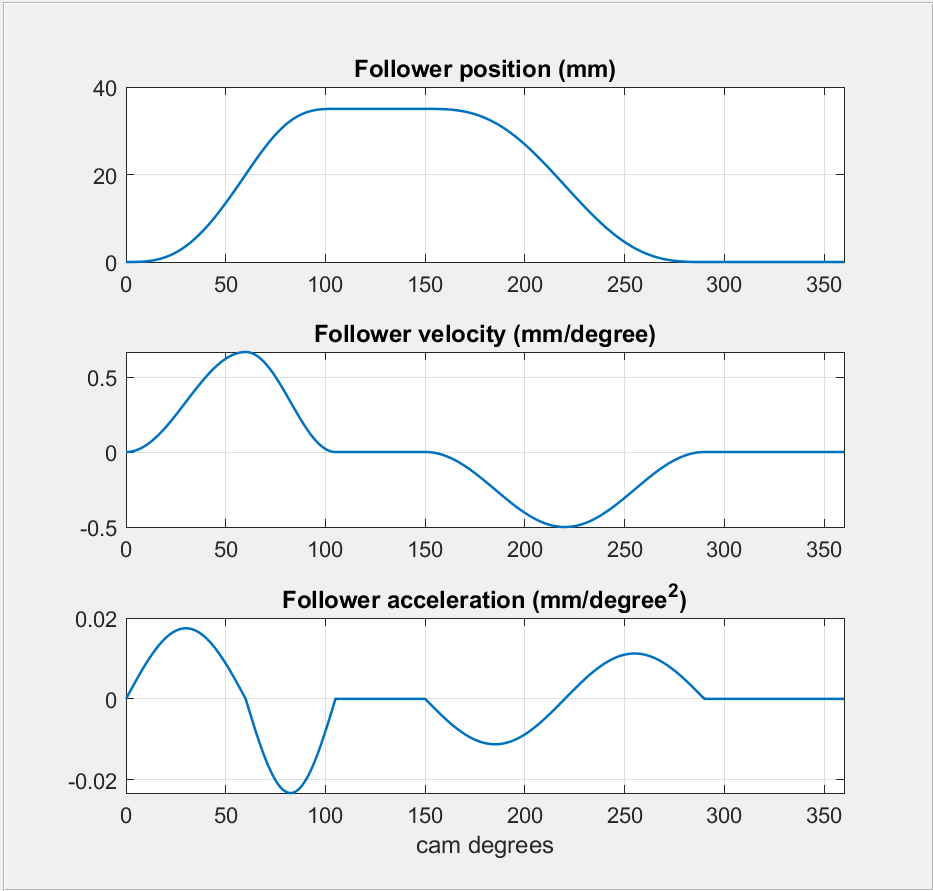
\includegraphics[width=.7\textwidth]{hefwet.png}
	\caption{The motion law \(S(\theta)\) and its first and second derivatives in function of the cam angle \(\theta\). These plots were created with \texttt{matcam.m}}
	\label{fig:hefwet}
	
\end{figure}

The chosen segment sequence for this system consists of a C1, a C2 and a C6 segment and some dwells (segment with no rise or decline, which leads to a constant displacement).

\begin{itemize}

\item The first segment is a C1 half-cycloid which rises from 0 to +20 millimeters between 0 and 60 degrees. 

\item The second one is a C2 half-cycloid that rises from +20 to +35 millimeters between 60 and 105 degrees. By choosing to end this segment at 105 degrees, the first derivative of S is perfectly continuous in \(\theta=60\degree\).

\item After this second half-cycloid comes a dwell at +35 millimeters between 105 and 150 degrees. This dwell forms a perfectly continuous funtion with the C2 half-cycloid before it and the decreasing C6 cycloid behind it.

\item The last cycloidal part is a C6 segment that declines from +35 to 0 millimeters between 150 and 290 degrees.

\item To connect the C6 cycloid back with the C1 segment, a dwell at 0 millimeters is used between 290 and 360 degrees.

\end{itemize}

A summary of these segments is given in table~\ref{tab:motionlaw}. A graphical representation of this motion law and of its first and second derivatives is shown in figure~\ref{fig:hefwet}. On this plot one can see that the velocity is perfectly continuous and that the absolute value of the acceleration does not exceed \(0,025~\si{mm/degree^2}\).

\begin{table}[h]
	\centering
	\resizebox{\textwidth}{!}{\begin{tabular}{c|cccc}
		Segment & \(\beta_{start}\) (degrees) & \(\beta_{end}\) (degrees) & Cycloid type & Relative displacement (mm) \\
		\hline
		1 & 0 & 60 & C1 & +20 \\
		2 & 60 & 105 & C2 & +15\\
		3 & 105 & 150 & dwell & 0\\
		4 & 150 & 290 & C6 & -35\\
		5 & 290 & 360 & dwell & 0\\
	\end{tabular}}
	\caption{Results of the use of the Kloomok and Muffley diagram for each segment with a lift \(L\neq0\).}
	\label{tab:motionlaw}
\end{table}

\section{Determining the geometry of the follower}
\label{sec:2}

Some geometric characteristics of the follower must be chosen wisely to optimize the cam's operation. The choice of these parameters is the subject of this section.

The radiuses of the base circle of the cam and of the follower's roller must be chosen so that there is no undercutting and that the pressure angle never exceeds 30 degrees. Then the excentricity can help to make the maximal pressure angle even smaller.

\subsection{Sum of the radiuses of base circle and follower, \(R_0\)}

First, the pitch circle radius \(R_0\) is calculated. This is the sum of the base circle radius \(R_{base}\) and the follower radius \(R_r\), the two variables that need to be found in this subsection. 

This can be done by looking at the pressure angle. This is the angle between the direction in which the follower translates and the normal on the cam's surface. It gives an indication of how the transmitted force between cam and follower is converted. When the pressure angle is small, most of this force will be used for the follower's motion. When the pressure angle is more right (\(\approx90\degree\), most of it will be converted in frictional forces. The latter case must of course be avoided. A good rule of thumb states that the pressure angle must never exceed 30 degrees:

\begin{equation}
	\alpha_{max} < 30 \degree 
\end{equation}

The Kloomok and Muffley nomogram on slide 33 of chapter 8 in the manual~\cite{cursus} gives the relation between the pressure angle \(\alpha\) and the ratio of the displacement to the pitch circle radius \(L/R_0\). For each segment of the motion law, a line is drawn in this nomogram between the point of \(\alpha=30 \degree\) (the maximal allowed value for \(\alpha\)) and the point of the \(\beta\) which represents the size in degrees of the considered segment. The intersection of this drawn line and the horizontal axis in the nomogram gives the \(L/R_0\) ratio for that cycloidal segment. An example of how to use the nomogram is given in figure~\ref{fig:nomogram1}.

The results for each segment are listed in table~\ref{tab:nomogram}. Because the displacement \(L\) is known for each segment, the pitch circle radius \(R_0\) can be calculated for each segment. The highest value for \(R_0\) is 60 millimeters. By choosing this value or higher, the pressure angle will surely not exceed 30 degrees. This will still be optimized by choosing an excentricity, so 60 millimeters is good enough for now.

\begin{figure}
	\centering
	\includegraphics[width=.66\textwidth]{nomogram1.png}
	\caption{Nomogram of Kloomok and Muffley used to determine the pitch circle radius \(R_0\).}
	\label{fig:nomogram1}
\end{figure}

\begin{table}
	\centering
	\begin{tabular}{c|cccc}
		Segment & \(\beta\) (degrees) & \(L\) (mm) & \(L/R_0\) & \(R_0\) (mm) \\
		\hline
		1 & 60 & 20 & 0,33 & 60 \\
		2 & 45 & 15 & 0,25 & 60\\
		4 & 35 & 35 & 0,90 & 39\\
	\end{tabular}
	\caption{Results of the use of the Kloomok and Muffley diagram for each segment with a lift \(L\neq0\).}
	\label{tab:nomogram}
\end{table}

\subsection{Radius of the base circle, \(R_{base}\) and radius of the follower, \(R_r\)}

The conclusion of the previous subsection was that \(R_{base}+R_r=60~mm\). Now the base circle radius and the follower radius must be determined seperately. This can be done by stating that to avoid undercutting, the radius of curvature of the cam's surface must always be greater than the follower radius:

\begin{equation}
	\rho _{min} > R_r
\end{equation}

To calculate this minimal radius of curvature, another nomogram of Kloomok and Muffley is used. It is generated by the MATLAB function \texttt{gen\_fig\_Kloomok\_Muffley.m}. This program makes plots of the \(\rho_{min}\) of each segment given the pitch radius \(R_0\), the lift and the cycloid type. These plots are listed in figure~\ref{fig:nomogram2}.

From these plots, one can see that the smallest value for \(\rho_{min}\) is 60 millimeters, which means that the follower radius must be smaller than 60 millimeters. This is just an upper boundary, so it can be a lot smaller than that. We have chosen to make \textbf{\(R_r=10~mm\)}, so that the base circle radius is \textbf{\(R_{base}=50~mm\)}. It is desirable that the follower radius is smaller than the base circle radius to make the motion smoother.

Plots of the pressure angle and the radius of curvature with these radiuses can be seen in figure~\ref{fig:geozonder}.

\begin{figure}
	\centering
	
	\begin{subfigure}{.7\textwidth}
		\centering
		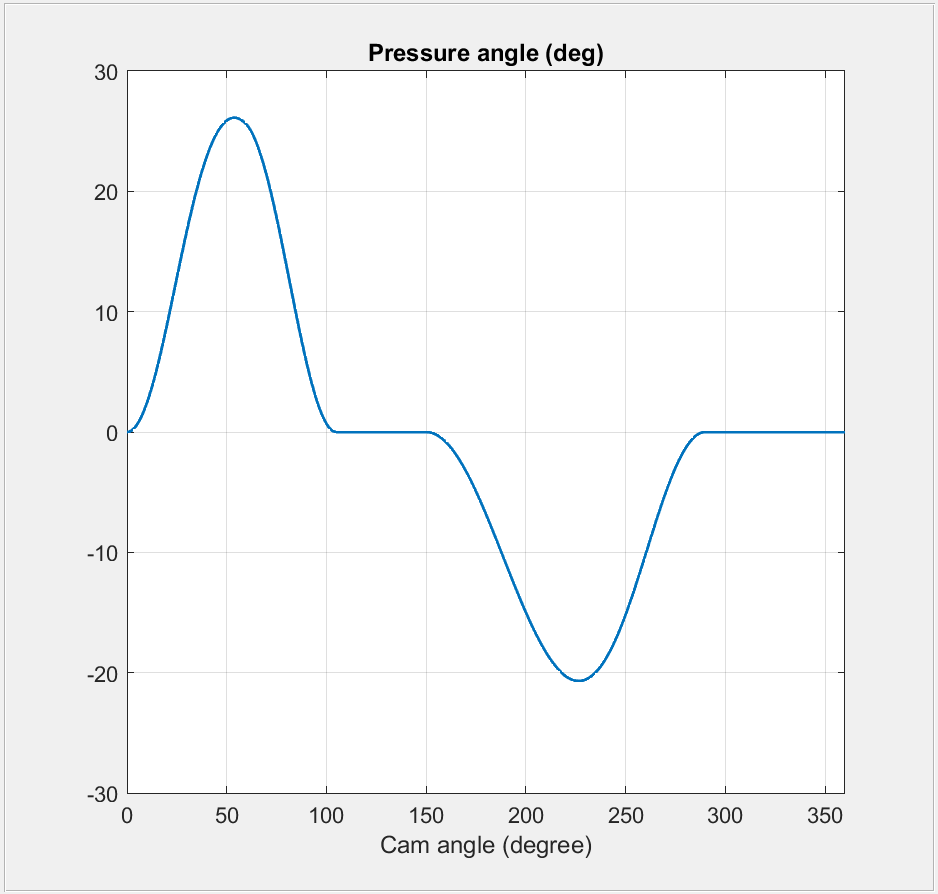
\includegraphics[width=\textwidth]{preszonder.png}
		\caption{Pressure angle in function of cam angle. For smooth motion, this angle must never exceed 30 degrees.}
		\label{fig:preszonder}
	\end{subfigure}
	\hfill
	\begin{subfigure}{.7\textwidth}
		\centering
		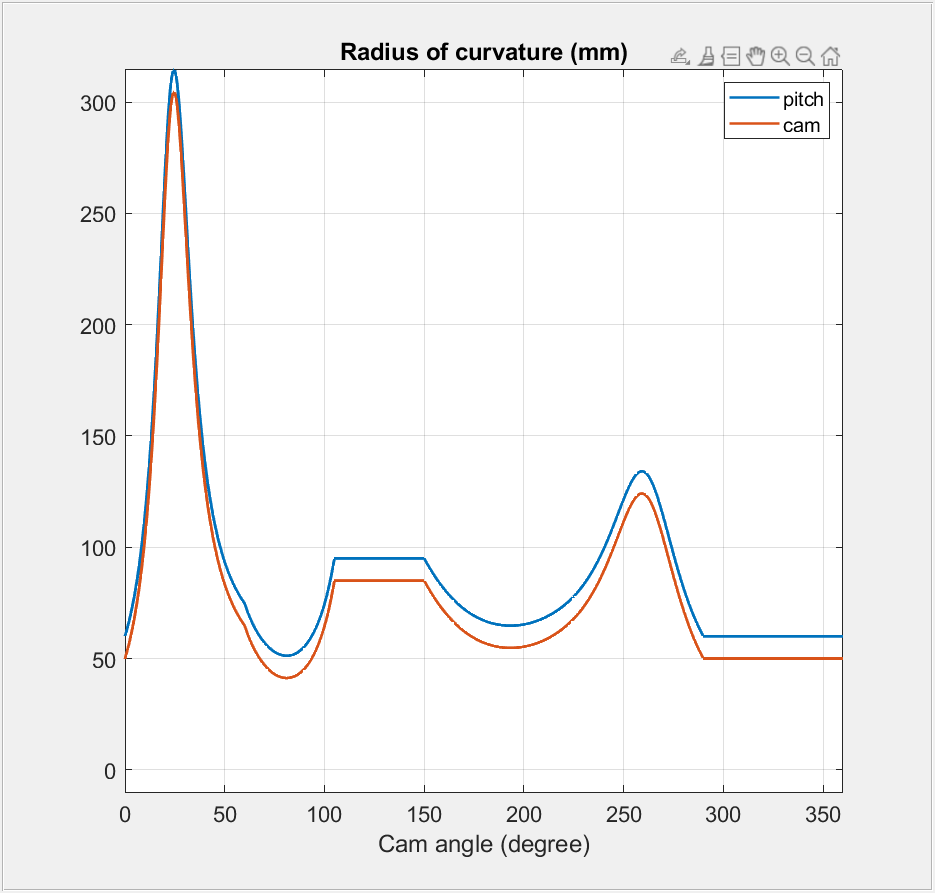
\includegraphics[width=\textwidth]{radzonder.png}
		\caption{Radius of curvature in function of cam angle. To avoid undercutting, the follower radius \(R_r\) must always be smaller than the pitch radius of curvature (blue line).}
		\label{fig:radzonder}
	\end{subfigure}
	
	\caption{Pressure angle \(\alpha\) and radius of curvature \(\rho\) in function of cam angle for the case of a centric follower with \(R_r=10~mm\) and \(R_{base}=50~mm\).}
	\label{fig:geozonder}
	
\end{figure}

\begin{figure}
	\centering
	
	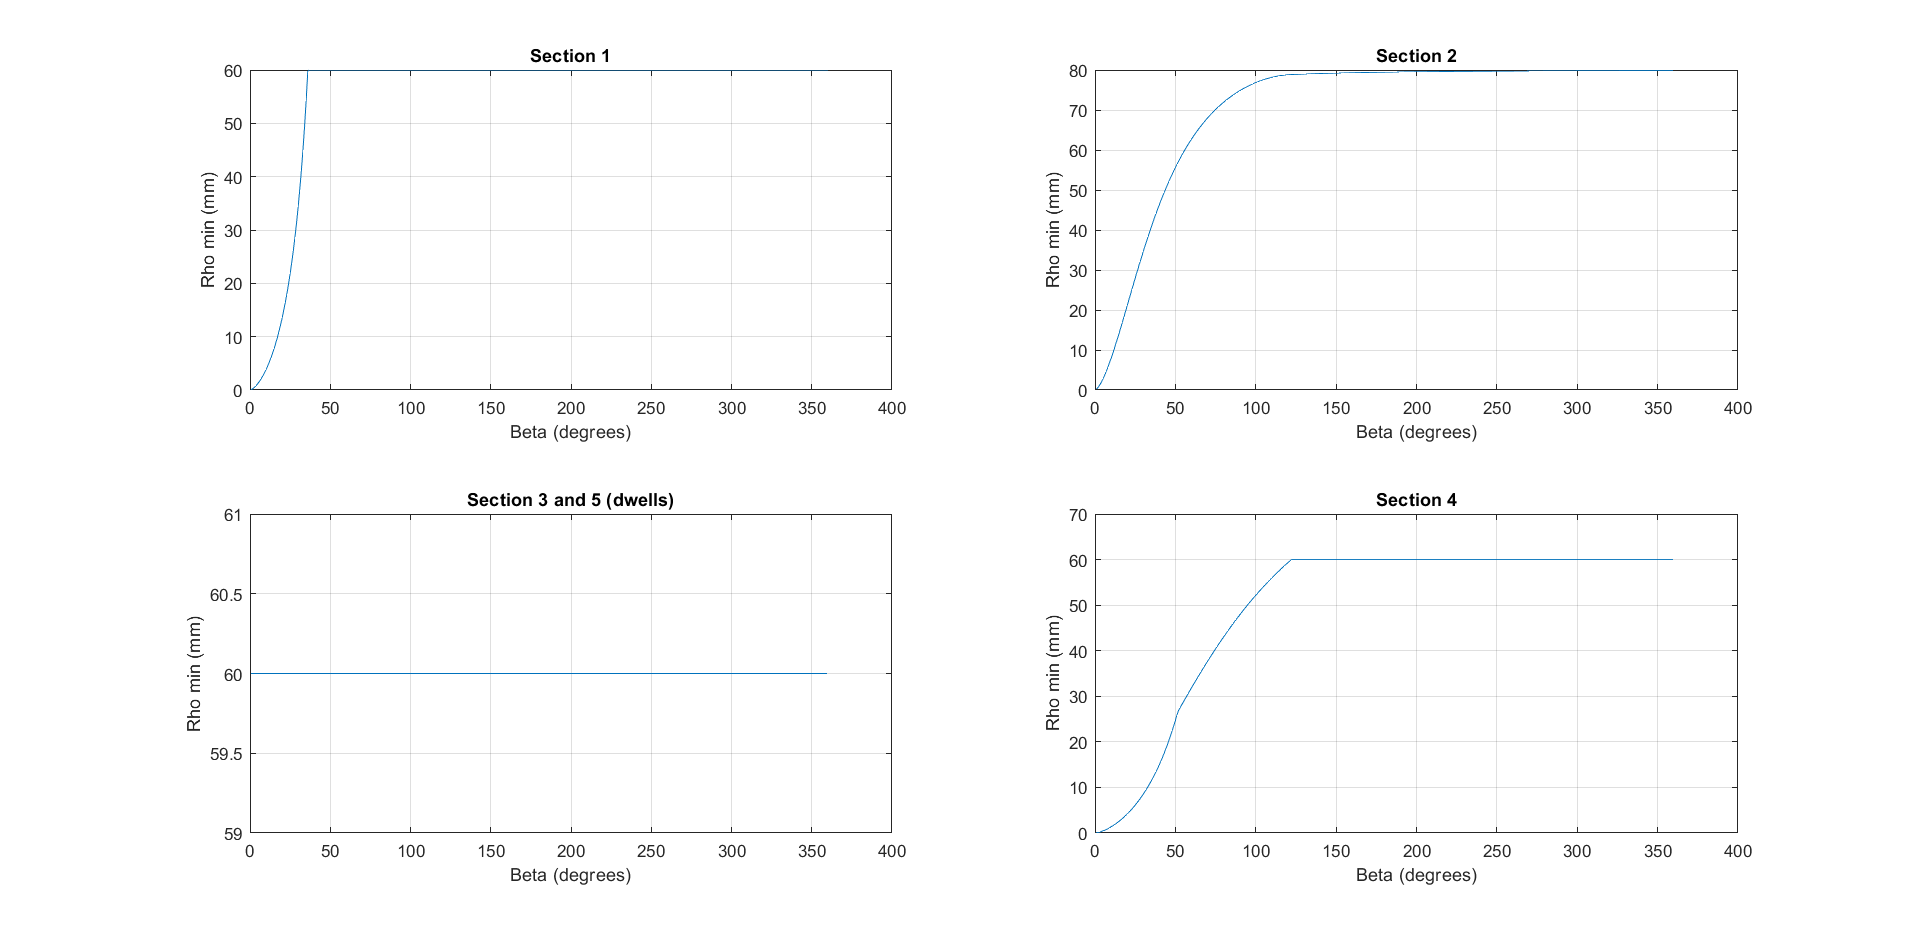
\includegraphics[width=\textwidth]{nomogram2.png}
	
	
	\caption{Nomograms of Kloomok and Muffley for determining the \(\rho_{min}\).}
	\label{fig:nomogram2}
\end{figure}

\subsection{Excentricity \(e\)}

In the previous subsections, the follower was assumed to be in line with the center of the cam. The follower can however also be placed excentrically relative to the cam. This can help to reduce the pressure angle.

When choosing an excentricity \(e\) different from zero, the curve of the pressure angle in function of the cam angle, which is plotted in figure~\ref{fig:preszonder}, moves up or down. The intention is to find an excentricity so that the maximal value and the minimal value of the pressure angle lie symmetrically relative to the horizontal axis. In that case, the maximal value for \(|\alpha|\) is minimized.

Finding the ideal excentricity was done by trial and error in \texttt{matcam.m}. For \textbf{\(e=4,5~mm\)} the pressure angle is optimal. It can be seen in figure~\ref{fig:presmet}. The new radius of curvature can be seen in figure~\ref{fig:radmet}.

\begin{figure}
	\centering
	
	\begin{subfigure}{.7\textwidth}
		\centering
		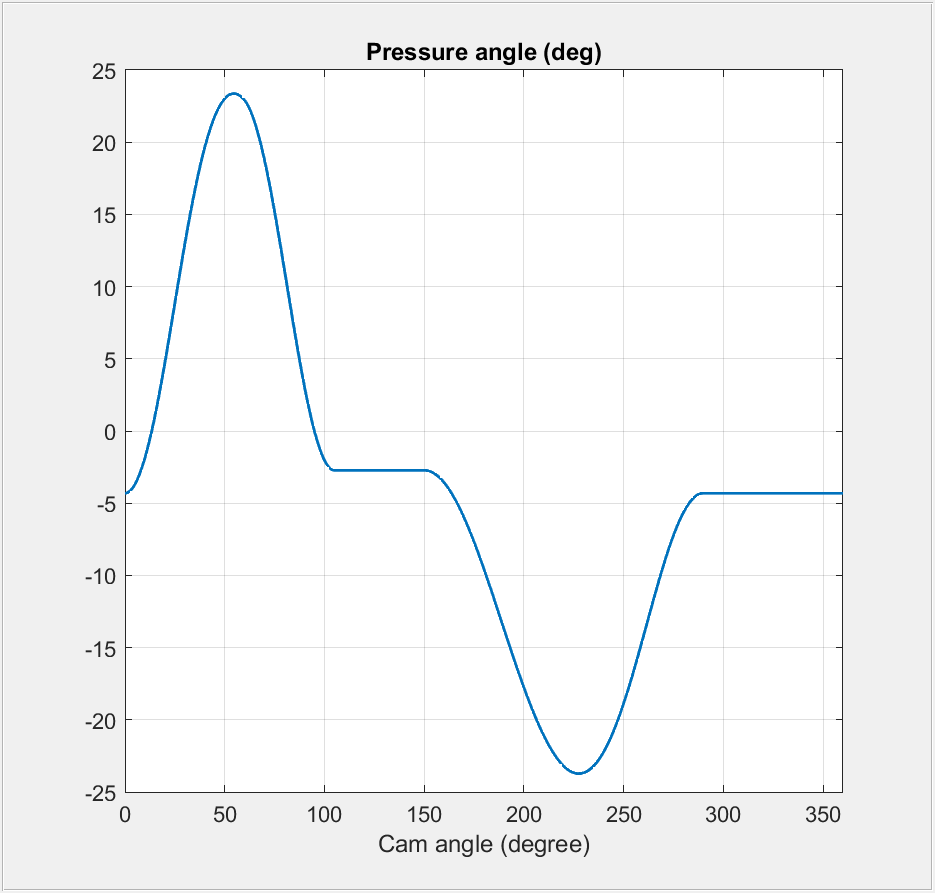
\includegraphics[width=\textwidth]{presmet.png}
		\caption{Pressure angle in function of cam angle. For smooth motion, this angle must never exceed 30 degrees.}
		\label{fig:presmet}
	\end{subfigure}
	\hfill
	\begin{subfigure}{.7\textwidth}
		\centering
		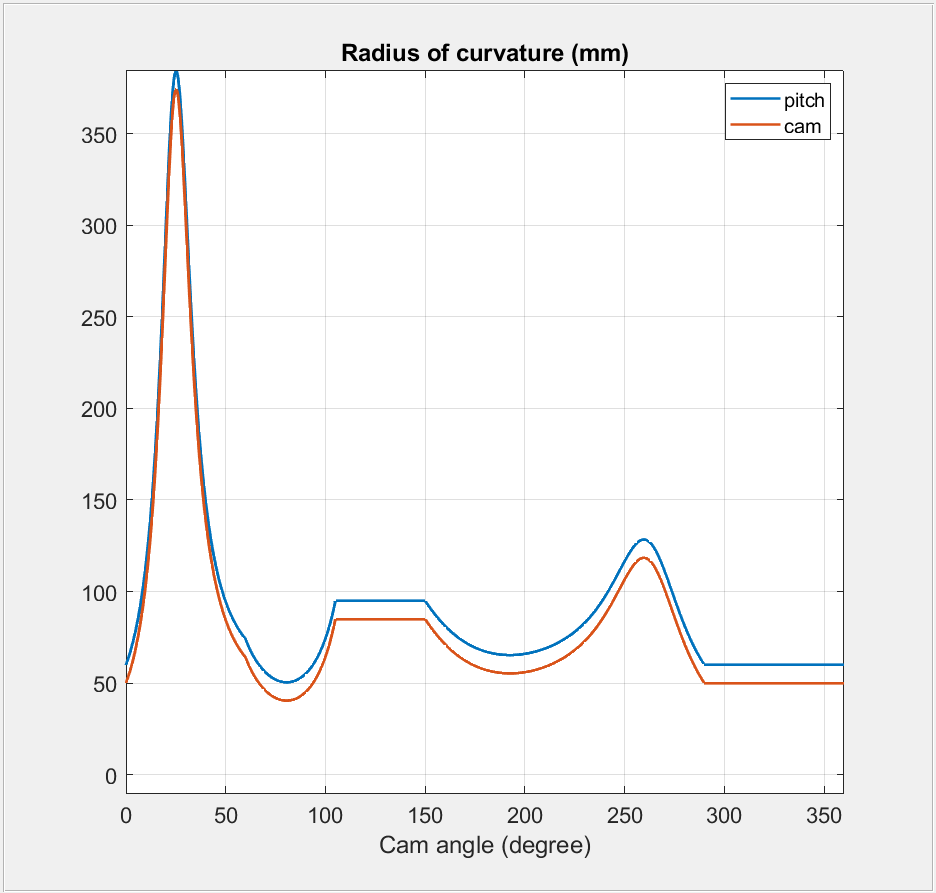
\includegraphics[width=\textwidth]{radmet.png}
		\caption{Radius of curvature in function of cam angle. To avoid undercutting, the follower radius \(R_r\) must always be smaller than the pitch radius of curvature (blue line).}
		\label{fig:radmet}
	\end{subfigure}
	
	\caption{Pressure angle \(\alpha\) and radius of curvature \(\rho\) in function of cam angle for the case of an excentric follower with \(R_r=10~mm\), \(R_{base}=50~mm\) and \(e=4,5~mm\).}
	\label{fig:geomet}
	
\end{figure}

\section{Verifying the rigid body forces}

\subsection{Sizing the spring}

\subsection{Instantaneous power}

The power to drive the cam is given for a non-excentric follower \cite{vermogen}:

\begin{equation}
	\begin{split}
	P(\theta) & = \vec{N}(\theta)\cdot\vec{v}(\theta) \\
	&=N(\theta)\cdot sin(\alpha)\cdot R(\theta)\cdot \omega
	\end{split}
\end{equation}

For the case where there is an excentrity \(e\neq0\), the power is calculated as follows:

\begin{equation}
	\begin{split}
	P(\theta) & = \vec{N}(\theta)\cdot\vec{v}(\theta) \\
	&=N(\theta)\cdot cos(\alpha)\cdot f'(\theta)\cdot\omega
	\end{split}
	\label{eq:verm_exc1}
\end{equation}

The pressure angle for a cam with an excentric follower is given in slide 31 of chapter 8 of the manual~\cite{cursus}: FIGUURFIGUURGIFURGIFURIFUFRIFUUUUUFFF

\begin{equation}
	\begin{split}
	\alpha& = arctan\left(\frac{f'(\theta)-e}{\sqrt{R_0^2-e^2}+f(\theta)}\right)\\
	&=arctan\left(\frac{f'(\theta)-e}{\sqrt{R(\theta)^2-e^2}}\right)
	\end{split}
	\label{eq:verm_exc2}
\end{equation}

And by using equation~\ref{eq:verm_exc2} in equation~\ref{eq:verm_exc1}, the power can be written as:

\begin{equation}
	\begin{split}
	P(\theta) =&~ N(\theta)\cdot cos(\alpha)\cdot \Big(tan(\alpha)\cdot\sqrt{R(\theta)^2-e^2}+e\Big)\cdot\omega\\
	=&~N(\theta)\cdot sin(\alpha)\cdot\sqrt{R(\theta)^2-e^2}\cdot\omega  +~N(\theta)\cdot cos(\alpha)\cdot e \cdot\omega
	\end{split}
\end{equation}

The power for both the case without excentricity and the case with excentricity (\(e=4,5~cm\) as determined in section~\ref{sec:2}) is calculated in the MATLAB function \texttt{power.m}. The plots of the powers in function of \(\theta\) can be found in figure~\ref{fig:powerplot}. Figure~\ref{diffpower} shows the difference between the two power plots. This difference is of an order of magnitude of \(10^{-14}\) and is due to the machine precision of MATLAB. The power for the cam with a centric follower is thus equal to the power for the cam with an excentric follower.

\begin{figure}
	\centering
	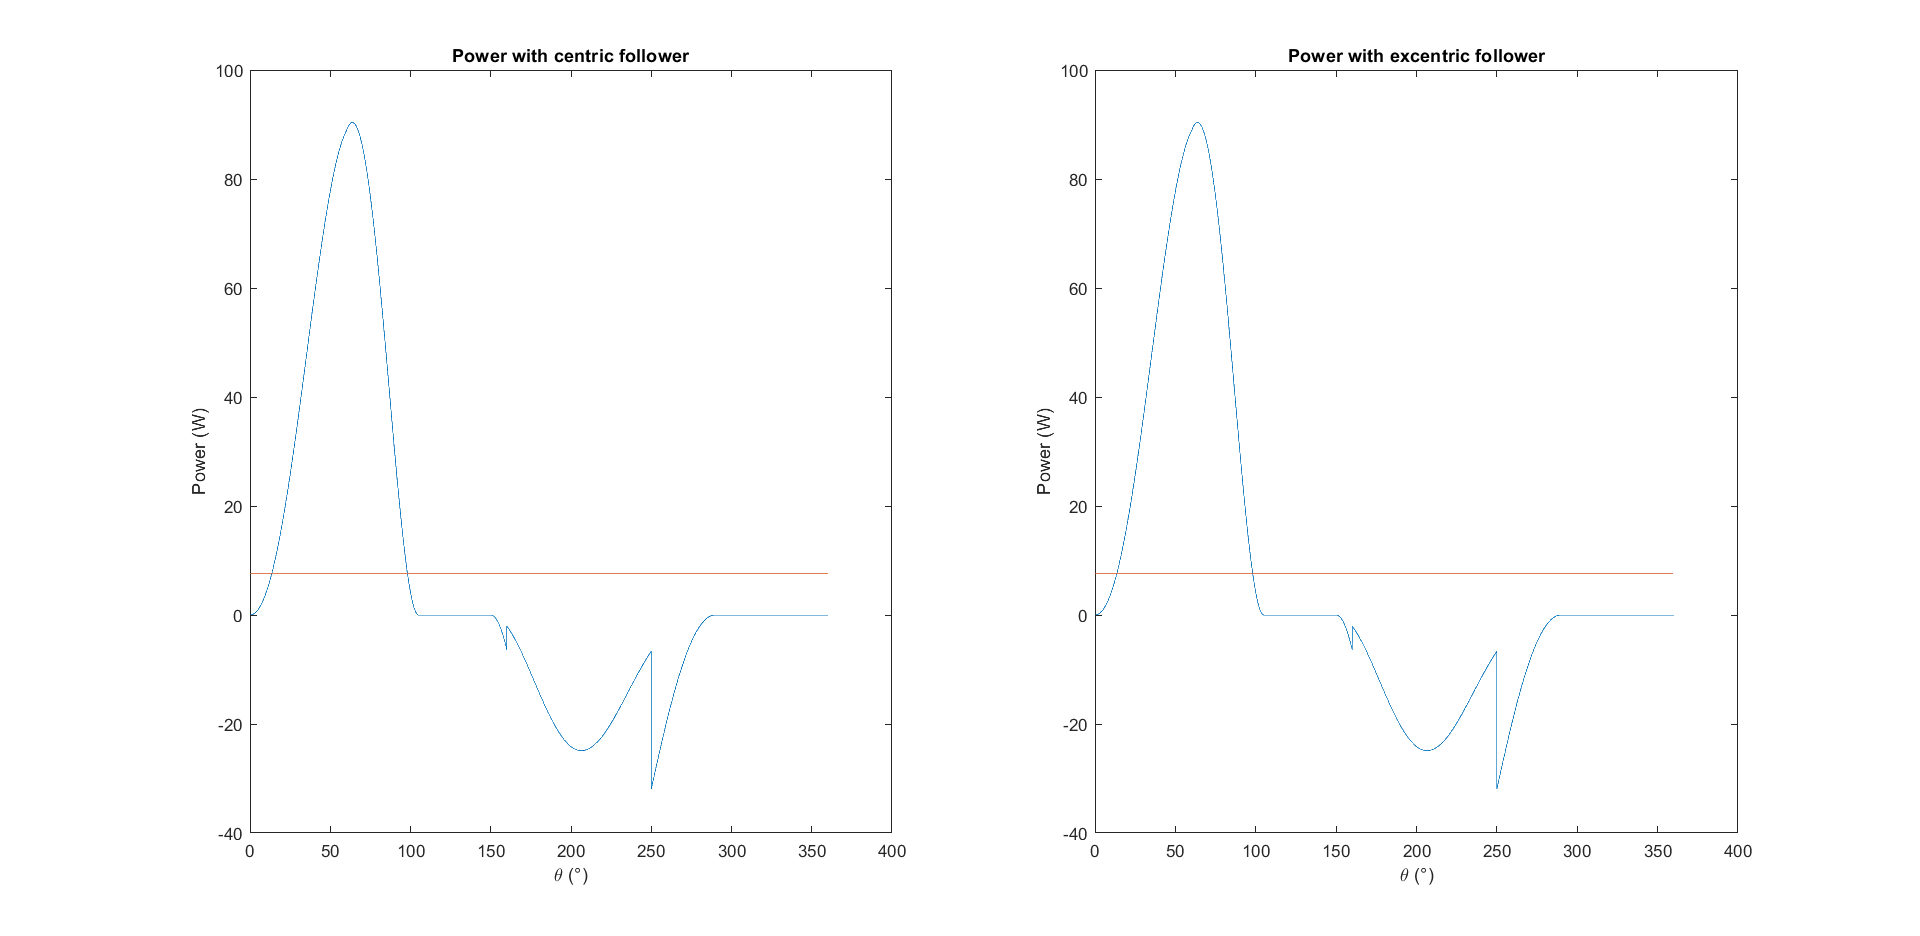
\includegraphics[width=\textwidth]{powerplot.png}
	\caption{The instantaneous power \(P\) to drive the cam in function of \(\theta\) for a centric and an excentric follower.}
	\label{fig:powerplot}
	
\end{figure}

\begin{figure}
	\centering
	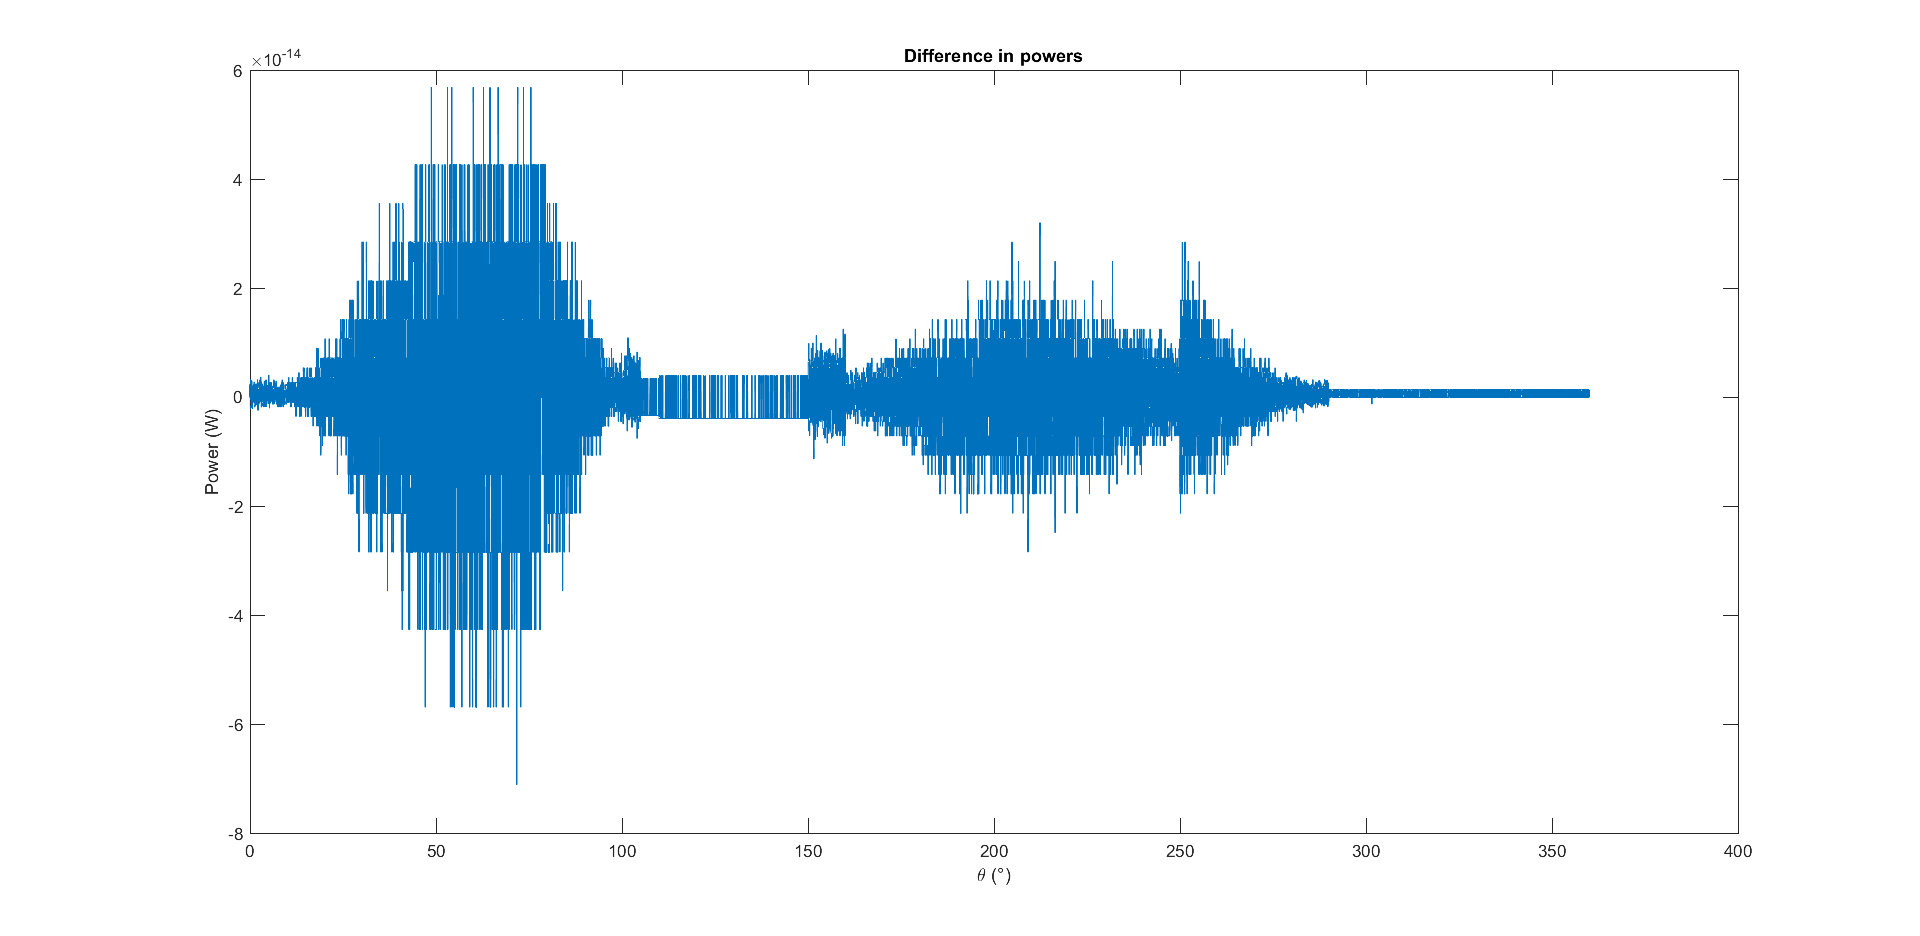
\includegraphics[width=\textwidth]{diffpower.png}
	\caption{Difference between the power with and without excentricity in function of \(\theta\).}
	\label{diffpower}
\end{figure}

\subsection{Designing a flywheel}

\section{Dynamics of the follower}

\bibliographystyle{plain}
\bibliography{nokken}

\end{document}